\newcommand{\plogo}{\fbox{$\mathcal{PL}$}} % Generic dummy publisher logo

%\usepackage[utf8]{inputenc} % Required for inputting international characters
%\usepackage[T1]{fontenc} % Output font encoding for international characters
%\usepackage{fouriernc} % Use the New Century Schoolbook font
\documentclass{article}[12pt]
\usepackage[margin=2.5cm]{geometry}
\usepackage{enumerate}
\usepackage{booktabs}
\usepackage{amsmath}
\newtheorem{theorem}{Theorem}  
\newtheorem{lemma}{Lemma}  
\usepackage{pifont}
\newtheorem{proof}{Proof}
\usepackage{caption}
\usepackage{amssymb}
\usepackage{ulem}
\usepackage{graphicx}
\usepackage{subfigure}
\usepackage{geometry}
\usepackage{multirow}
\usepackage{multicol}
\usepackage{indentfirst}
\usepackage{xcolor}
\usepackage{verbatim}
%\usepackage{ctex}
\usepackage{gauss}
\usepackage{float}
\usepackage[version=4]{mhchem}

\begin{document}
\noindent

%========================================================================
\noindent\framebox[\linewidth]{\shortstack[c]{
\Large{\textbf{VE203 Assignment 3}}}}
\begin{center}
\footnotesize{\quad Name: YIN Guoxin\quad Student ID: 517370910043}


\end{center}
%=======================================================================

\noindent \textbf{Q1.}
\begin{enumerate}[(i)]
\item According to the definition of $[a,b]$, all the elements in this set is also contained in $L$. Since $(L,\preceq)$ is a complete lattice, $(l,\preceq)$ must be a lattice and therefore also a poset. Therefore, $([a,b],\preceq )$ must also be a poset since all the element containing in it satisfies the prerequisite for a set to be a lattice and a poset. Therefore, for all non-empty set $[c,d]\subseteq [a,b]$, since for $\forall y\in [c,d]$, we have $c\preceq y\preceq d$, which means $c\in [a,b]$ is the g.l.b and $d\in [a,b]$ is the l.u.b of $[c,d]$. Besides, as for the empty set, we first have all $z\in [a,b]$ is both the u.b and l.b of $\emptyset$. And then we know that $\forall z\in [a,b], z\preceq b$ and $a\preceq z$, $a,b\in [a,b]$, which means that $b$ is the g.l.b and $a$ is the l.u.b of $\emptyset$. Therefore, every $X\subseteq [a,b]\subseteq L$ has both a l.u.b. and a g.l.b, which means that $([a,b],\preceq )$ is a complete lattice.
\item For $\forall x\in S$, since $S\subseteq X$, $x\in X$. And $a\in X$ is the element that for all $y\in X$, $a\preceq y$. Therefore, we have $a\preceq x$ for all element $x\in S$. Therefore, $a$ is one lower bound of the set $S$. However, we also know that $s$ is the g.l.b of $S$. Therefore, we must have $a\preceq s$.
%\item Since $[a,s]$ is defined by (i), we know that it is a complete lattice. Suppose there exist elements in $[a,s]$ that is also in $X$ and denote the set of those elements as $Y$. And particularly, suppose there exist several elements $n_i\in Y$, such that for any \textbf{other} elements $y$ in $Y$ (i.e. $y$ is different from all $n_i$), $y\preceq n_i$.\par
%Then, since $f$ is order-preserving and $s\preceq z,\forall z\in S$, we have $f(s)\preceq f(z),\forall z\in S$, which means $f(s)$ is also a lower bound of $S$. But $s$ is the g.l.b of $S$, therefore $s\preceq f(s)$. From the fact that $f$ is order-preserving, we then have $s\preceq f(s)\preceq f(f(s))\preceq f(f(f(s)))......$ and so on.
%\par Also since $f$ is order-preserving and $a\preceq n_i\ (i.e. n_1,n_2,...)\preceq s$, we have $a=f(a)\preceq f(n_i)=n_i\preceq f(......f(f(f(s))))\preceq ... \preceq f(s)\preceq s$. Therefore, since the number of $'f'$ in $f(......f(f(f(s))))$ can be infinite, we cannot find a l.u.b of the various $n_i$, which breaks the fact that $[a,s]$ is a complete lattice.
\item \begin{itemize}
\item We first need to prove that if $(L,\preceq)$ is a complete lattice, and $f:(L,\preceq)\Rightarrow (L,\preceq )$ is an order-preserving function, then $f$ has a greatest fixed point. Consider 
\begin{align*}
Y=\{y\in L| y\preceq f(y)\}\ \rm{and}\ b=\bigvee Y
\end{align*}
\textbf{Claim I:} If $y\in Y$, then $f(y)\in Y$. To see this, let $y\in Y$. Therefore, $y\preceq f(y)$. Since $f$ is order preserving, $f(y)\preceq f(f(y))$. This shows that $f(y)\in Y$.\\
\textbf{Claim II:} $ f(b) $ is an upper bound on $Y$. To see this, let $y\in Y$. Therefore, $y\preceq b$, since $b$ is an upper bound on $Y$. Since $f$ is order-preserving, $f(y)\preceq f(b)$. Since $y\preceq f(y)$, it follows that $y\preceq f(b)$. \par
It follows from Claim II that $b\preceq f(b)$, because $b$ is the l.u.b of $Y$. Therefore, $b\in Y$. So, by Claim I, $f(b)\in Y$. Therefore, $f(b)\preceq b$ and $b=f(b)$. So $b$ is a fixed point of $f$.\par 
Since for any fixed point $x$, $f(x)=x$, by the reflexive property, we must have $x\preceq x =f(x)$. Therefore, all the fixed points are in $Y$. Since $b$ is the upper bound of $Y$ and $b\in Y$, $b$ must be the greatest fixed point because any fixed point $x\preceq b$.
\item From the question (i), we know that $([a,s],\preceq)$ is a complete lattice. Then, since $f$ is order-preserving and $s\preceq z,\forall z\in S$, we have $f(s)\preceq f(z),\forall z\in S$, which means $f(s)$ is also a lower bound of $S$. But $s$ is the g.l.b of $S$, therefore $s\preceq f(s)$. Also since $f$ is order-preserving and $a\preceq x\preceq s$ for any $x\in[a,s]$, we have $a=f(a)\preceq f(x)\preceq  f(s)\preceq s$, which means when the domain of $f$ is $[a,s]$, range of $f \subseteq [a,s]$.
Therefore, there must exist a greatest fixed point among all the fixed points in $[a,s]$, and we denote it as $s_X$. Since $s_X\in [a,s]$, we have $s_X\preceq s$. Since $s$ is the g.l.b of $S$, for $\forall x\in S$, we have $s\preceq x$. Therefore, we have $\forall x\in S, s_X\preceq x$ due to transitive property. Since for any other fixed point $t$ in $[a,s]$ we have $t\preceq s_X$ and thus $s_X$ must be the g.l.b of $S$ in $X$. 
\end{itemize}
\item First, by Tarski-Knaster Theorem, we denote the least fixed point in $X$ as $a$ and the greatest fixed point n $X$ is $b$.
\begin{itemize}
\item For $\emptyset$, its l.u.b is $a$ since all the fixed points is its upper bound and $a \preceq x, forall x\in X$. Similarly, its g.l.b is $b$ since all the fixed points is its least bound and $\forall x\in X, x\preceq b$.
\item For every non-empty subset of $X$ (denote as $X_s$), it is also a subset of $L$, therefore, it must have a g.l.b (denoted as $c\in L$) and a l.u.b (denoted as $d\in L$) in $L$. Therefore, by question (i), we know that $[c,d]$ is also a complete lattice, therefore, there are must exist a greatest fixed point and a least fixed points among all fixed points in $[c,d]$, and the former one is of course the only upper bound (i.e. l.u.b) of $X_s$ and the latter one is the only lower bound (i.e. g.l.b) of $X_s$.
\end{itemize}
\item The expression for $f$ is shown below as well as its graph.
\begin{equation*}
f(x)=
\begin{cases}
2x& 0\leq x< \frac{1}{8}\\
\frac{1}{4}& \frac{1}{8}\leq x< \frac{1}{4}\\
2x-\frac{1}{4}&	\frac{1}{4}\leq x< \frac{1}{2}\\
\frac{3}{4}& \frac{1}{2}\leq x< \frac{3}{4}\\
2x-\frac{3}{4}&	\frac{3}{4}\leq x< \frac{7}{8}\\
1& \frac{7}{8}\leq x\leq 1\\
\end{cases}
\end{equation*}
\begin{figure}[H]
\centering
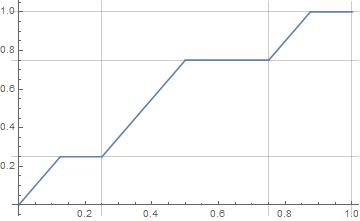
\includegraphics [width=9cm,height=5cm]{1_5.jpg}
\end{figure}
\end{enumerate}





\noindent \textbf{Q2.}
\begin{enumerate}[(i)]
\item 
\begin{itemize}
\item We first prove that $(X\subseteq)$ is a poset.
\begin{enumerate}
\item It is reflexive since every set is the subset of itself.
\item It is antisymmetry since for any two set $A,B$ if $A\subseteq B$ and $B\subseteq A$, they must be equal.
\item It is transitive. For any three set $A,B,C$, if $A\subseteq B$ and $B\subseteq C$, we must have $A\subseteq C$.
\end{enumerate}
\item For any subset $S\subseteq X$, we can always find $\bigwedge S=\bigcup S$ and $\bigvee S=\bigcap S$. Therefore, $(X\subseteq)$ is a complete lattice.
\end{itemize}
\item Suppose $A,B\subseteq X$ and $A\subseteq B$. Since all elements in $A$ must in $B$ but there exists element in $B$ that is not in $A$, we have $G``A\subseteq G``B$. Therefore, we have $F(A)=A\cup G``A\subseteq F(B)=B\cup G``B$. Therefore, $F$ is an order preserving function on ($X,\subseteq$).
\item \begin{itemize}
\item We first know that 0$\in $ dom($f$).
\item For any $k,m_k\in \mathbb{N},k\geq 0$, suppose $(m,k)\in f$ (i.e. $k\in \rm{dom}(f))$. Therefore, since $f$ is a fixed point of $F$, we have $f=F(f)=f\cup G``f$. Since $k\in$ dom($f$), $G((k,m_k))=(k+1,2^{m_k})\in G``f$. Therefore, $k+1\in \rm{dom}(f)$. 
\item In this way, we prove that all natural numbers must be in the domain of $f$.
\item Since $f\in \mathcal{P}(\mathbb{N}\times \mathbb{N})$, the domain of $f$ can only take values from $\mathbb{N}$, we have dom($f)=\mathbb{N}$.
\end{itemize} 

\item Since $ f(n) $ is the result of the power of 2, where the power is equal to $f(n-1)$, we only need to guarantee that $f(n-1)$ is a positive integer. 
\begin{itemize}
\item First, we know $G(0,0)=(1,1)$, $G(1,1)=(2,2)$. Since $G(1,1)\in G``f$, we have $G(1,1)\in f$. We can see that $f(1)=1$ is a positive integer, therefore, $f(2)=2^1=2$ is even.
\item Let $n\in \mathbb{N}$ with $n\geq 2$ and assume that $f(n)$ is a positive integer. Therefore, $f(n+1)=2^{f(n)}$ is also a positive integer and also an even number. 
\item Therefore, for all $n\in \mathbb{N}, n\geq 2$, f(n) is even.
\end{itemize}
\item Suppose that $f$ is not injective, which means there exists $a,b\in \mathbb{N},\ a\not=b$ such that $(a,m)\in f$ and $(b,m)\in f$. 
\begin{itemize}
\item Suppose $a$ or $b$ is zero, one from $(a,m)$ and $(b,m)$ must be (0,0), therefore, assume $(a,m)=(0,0)$, consider $f`=f/(b,m)$, then $f`\subseteq f$, which is against the fact that $f$ is the $\subseteq-$least in $X$.
\item Suppose neither $a$ nor $b$ is zero. Since $f$ is $\subseteq-$least, there exists a unique pair $(n,\log_2m)\in f$. Then apply $G$, we can only get one from $(a,m)$ and $(b,m)$. Then consider $f`=f/(b,m)$, then $f`\subseteq f$, which is against the fact that $f$ is the $\subseteq-$least in $X$.
\end{itemize}
Therefore, $f$ is injecive.
\end{enumerate}

\noindent \textbf{Q3.}
We first consider choosing elements one by one, when choosing the first element from the $n$ elements, we have $n$ choices. Continue choosing, when choosing the $i$th element from the rest $n-i+1$ elements, we have $n-i$ choices. Because we need to choose $k$ elements in total, we end up choosing after finishing choosing the $k$th element. Therefore, during choosing those elements, we have $n(n-1)(n-2)...(n-k+1)=\frac{n!}{(n-k)!}$. However, since if we choose the $k$ elements out of $n$ at the same time, we don't need to consider the order of them. Therefore, we need to factor out the ways to place $k$ elements in order, which is the number of bijections from $[k]$ to $[k]$, i.e. $k!$.\par
Therefore, we have 
\begin{align*}
\binom{n}{k}	=\frac{n!}{(n-k)!k!}
\end{align*}


\noindent \textbf{Q4.}
Since $(x+y)^n=\sum\limits_{k=0}^n\binom{n}{k}x^{n-k}y^k$, let $x=1$, $y=-1$, we have
\begin{align*}
0=(1+(-1))^n=\sum_{k=0}^n\binom{n}{k}1^{n-k}(-1)^k=\sum_{k=0}^n(-1)^k\binom{n}{k}
\end{align*}



\noindent \textbf{Q5.}
\begin{align*}
\binom{m+n+1}{m+1}&=\binom{m+n}{m}+\binom{m+n}{m+1}\\
&=\binom{m+n}{m}+\binom{m+n-1}{m}+\binom{m+n-1}{m+1}\\
&=......\ \rm{(keep\ making\ the\ last\ term\ into\ two\ terms\ with\ m\ and\ m+1\ at\ the\ bottom)}\\
&=\binom{m+n}{m}+\binom{m+n-1}{m}+...+\binom{m+1}{m}+\binom{m+1}{m+1}\\
&=\binom{m+n}{m}+\binom{m+n-1}{m}+...+\binom{m+1}{m}+\binom{m}{m}\\
&=\sum_{k=0}^{n}\binom{m+k}{m}
\end{align*}


\noindent \textbf{Q6.}
\begin{align*}
\left((x+y)^{8}+y\right)^{7}
&=\sum_{m=0}^7\binom{7}{m}((x+y)^8)^{7-m}y^m\\
&=\sum_{m=0}^7\binom{7}{m}(x+y)^{56-8m}y^m\\
&=\sum_{m=0}^7\binom{7}{m}(\sum_{k=0}^{56-8m}\binom{56-8m}{k}x^{56-8m-k}y^k)y^m\\
\end{align*}
Therefore, to make $56-8m-k=31$ and $k+m=4$, we have $k=1,m=3$. Therefore, the coefficient is $\binom{7}{3}\times \binom{56-24}{1}=1120$.\\


\noindent \textbf{Q7.}
\begin{align*}
(1+4\times \frac{1}{3})^{9}&=\sum_{k=0}^{9}\binom{9}{k}1^{9-k}(\frac{4}{3})^k\\
&=\sum_{k=0}^{9}\frac{9!}{k!(9-k)!}(\frac{4}{3})^k\\
\end{align*}
Suppose the greatest term is the $i+1$th (if we can find an integer solution $i$, it is not necessary for us to check whether $i$ is the first or the last term) term, $0\leq i\leq 9$. Then we must have 
\begin{align*}
&\frac{9!}{i!(9-i)!}(\frac{4}{3})^i\geq\frac{9!}{(i+1)!(8-i)!}(\frac{4}{3})^{(i+1)}\\
&\frac{9!}{i!(9-i)!}(\frac{4}{3})^i\geq\frac{9!}{(i-1)!(10-i)!}(\frac{4}{3})^{(i-1)}
\end{align*}
Through calculation, we find that $4.7\leq i\leq 5.71$. Therefore, $i=5$ and the greatest term is $\frac{9!}{5!(9-5)!}(\frac{4}{3})^5=$530.96.\\

\noindent \textbf{Q8.}The number of solutions is
\begin{align*}
\sum_{r=0}^6\binom{4+r-1}{r}&=\binom{3}{0}+\binom{4}{1}+\binom{5}{2}+\binom{6}{3}+\binom{7}{4}+\binom{8}{5}+\binom{9}{6}\\
&=1+4+10+20+35+56+84\\&=210
\end{align*}
\noindent \textbf{Q9.}
\begin{align*}
1.2^5=(1+0.2)^n&=\sum_{k=0}^5\binom{5}{k}1^{n-k}(0.2)^k\\
&=\sum_{k=0}^5\binom{5}{k}(0.2)^k\\
&=2.48832
\end{align*}

\noindent \textbf{Q10.}
\begin{enumerate} [(i)]
\item Suppose there exists $n \in \mathbb{N}_{\text { def }}$ with $n \neq \emptyset$ such that there doesn't exist $m \in \mathbb{N}_{\mathrm{def}}$ such that $n=S(m)$, which means $n\in \mathbb{N_{\text { def }}}$ but $n\not\in S``\mathbb{N_{\text { def }}}$. Because $S``\mathbb{N_{\text { def }}}\cup \mathbb{N}_{\mathrm{def}}=\mathbb{N}_{\mathrm{def}}$, we have $S``\mathbb{N_{\text { def }}}\subseteq \mathbb{N}_{\mathrm{def}}$. Given that $n\not\in S``\mathbb{N_{\text { def }}}$, we also have $S``\mathbb{N_{\text { def }}}\subseteq \mathbb{N}_{\mathrm{def}}/\{n\}$.

Therefore, consider $X=\mathbb{N}_{\rm{def}}/\{n\}$. We then have  $S``\mathbb{N_{\text{ def }}}\subseteq X$, which means $X\cup S``\mathbb{N_{\text{ def }}}=X$, which is against the fact that $\mathbb{N}_{\text{ def }}$ is the least fixed point for this operation.
\item 
\begin{enumerate}
\item For every non-empty subset $A\subseteq \mathbb{N}_{\text{ def }}$ except itself, it is finite. Since it is linear order, it is also well-order, which means we can find a least element in that set.
\item For $\mathbb{N}_{\text{ def }}$ itself, we can see that the element $\emptyset\in \mathbb{N}_{\text{ def }}$ can satisfy the quality that for all $x\in \mathbb{N}_{\text{ def }}$, if $x\leq \emptyset$, then $x=\emptyset$. To see this, we need to prove that for all $x\in \mathbb{N}_{\text{ def }}$, if $x\leq \emptyset$, then $x=\emptyset$.
\par If $x\leq \emptyset$, then there exists sets $A,B$ and $k\in \mathbb{N}_{\text{ def }}$, such that $A\cup B=\emptyset$, $|A|=|x|$ and $|B|=|k|$, and $|A\cup B|=|\emptyset|$. Therefore, $A\cup B=\emptyset$ since if there is a bijection from one set to the empty set, this set must also be the empty set. Therefore, we get $A,B=\emptyset$ and thus $x,k=\emptyset$ and we are done.
\end{enumerate}





%For every non-empty subset $A\subseteq \mathbb{N}_{\text{ def }}$, we can find $\bigcap A$, it must exist in A since every element in $ \mathbb{N}_{\text { def }}$ must contain the element ahead of it. Therefore, $\bigcap A$ is just the first element of $A$. And then we prove that for all $x\in A$, if $x\leq \bigcap A$, then $x=\bigcap A$.\\
%For all $x\in A$, if $x\leq \bigcap A$, then there exists sets $A,B$, such that $A\cup B=\
\end{enumerate}








%========================================================================
\end{document}
